\section{PID design}%
\label{closedloopyy}

Implementation of PID controller on the inverted pendulum. System parameters same as previous. \\
A unit impulse is applied to the system at $t = 0$. With determined parameters of $Kp = 1000, Ki = 100, Kd=10$ the output of the system, angle($\theta$), remains within the -5 to 5 degree requirement and angle is below 0.1$^\circ$ after 0.4s.

\begin{figure}[H]
	\centering
	\captionsetup{justification=centering}
	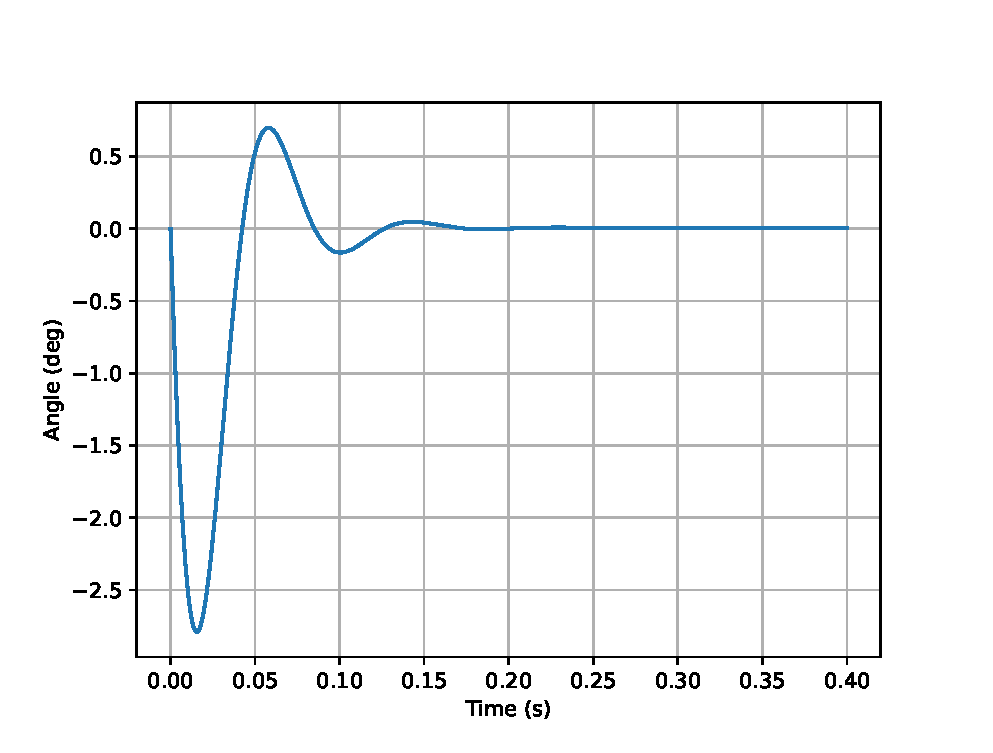
\includegraphics[width=0.8\linewidth]{imgs/q5_theta_t.eps}
	\caption{Force over time}%
	\label{fig:14}
\end{figure}
